\documentclass{standalone}
\usepackage{tikz}

\begin{document}
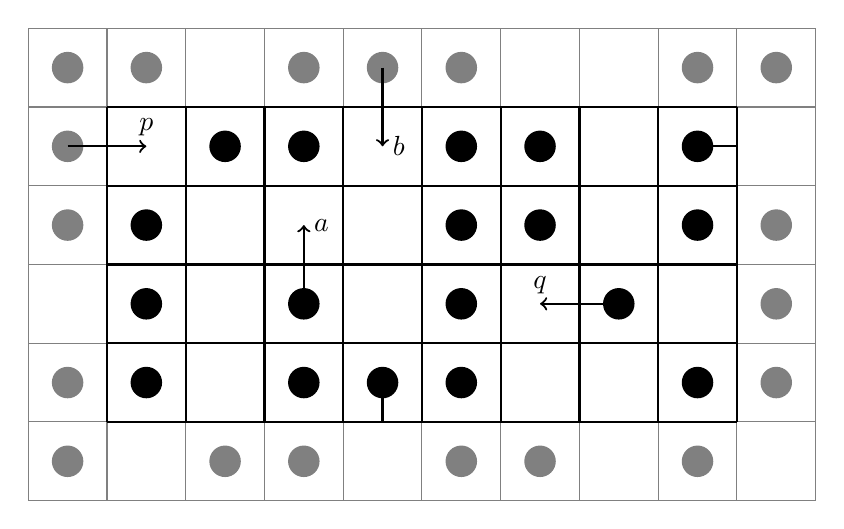
\begin{tikzpicture}
  % Grid
  \draw[step=1,gray, thin] (-1,-1) grid (9,5);
  \draw[step=1, thick] (0,0) grid (8,4);


  % Randomly placed particles
  \foreach \x in {1,3,4,5,8}
        \fill (\x-0.5,1-0.5) circle (0.2);
\foreach \x in {1,3,5,7}
    \fill (\x-0.5,2-0.5) circle (0.2);
\foreach \x in {1,5,6,8}
    \fill (\x-0.5,3-0.5) circle (0.2);
\foreach \x in {2,3,5,6,8}
    \fill (\x-0.5,4-0.5) circle (0.2);

  % Periodic boundary conditions
  % continue grid on all sites in gray
    \foreach \x in {0,2,3,5,6,8}
        \fill[gray] (\x-0.5,0-0.5) circle (0.2);
    \foreach \x in {0,1,3,4,5,8,9}
        \fill[gray] (\x-0.5,5-0.5) circle (0.2);
    \foreach \y in {1,3,4}
        \fill[gray] (0-0.5,\y-0.5) circle (0.2);
    \foreach \y in {1,2,3}
        \fill[gray] (9-0.5,\y-0.5) circle (0.2);

    % Arrows
    \draw[->, thick] (2.5,1.5) -- (2.5,2.5) node[right] {$a$};
    \draw[->, thick] (6.5,1.5) -- (5.5,1.5) node[above] {$q$};
    \draw[-, thick] (7.5,3.5) -- (8,3.5);
    \draw[->, thick] (-0.5,3.5) -- (0.5,3.5) node[above] {$p$};
    \draw[-, thick] (3.5,0.5) -- (3.5,0);
    \draw[->, thick] (3.5,4.5) -- (3.5,3.5) node[right] {$b$};

\end{tikzpicture}
\end{document}